如图~\ref{fig:arlac_calibrator_geometry} 所示，新候选参考源与 AR Lac 的角距离显著小于以往相位参考源。
\begin{figure}[htbp]
  \centering
  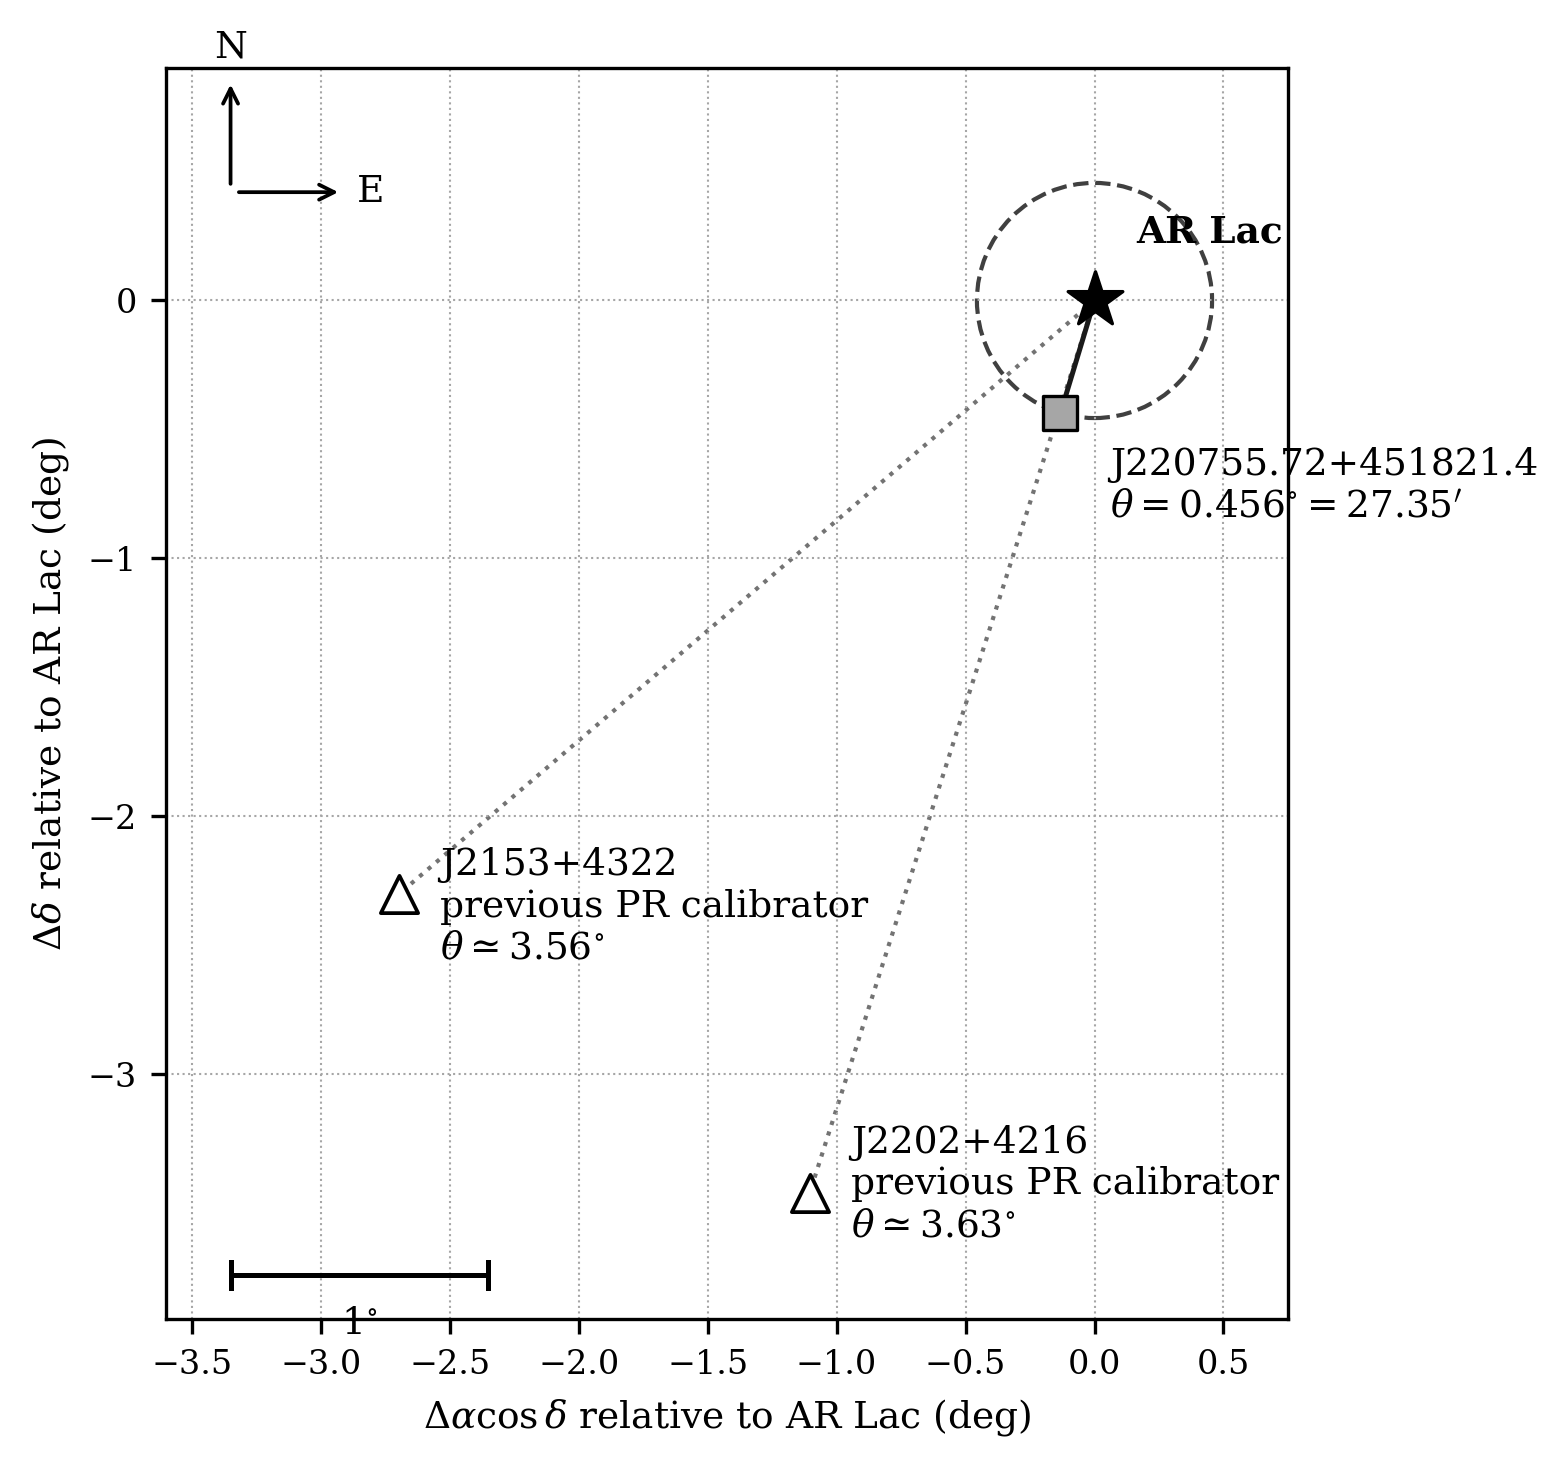
\includegraphics[width=0.60\linewidth]{imgs/arlac_calibrator_geometry.png}
  \caption{AR Lac 与候选近场参考源的相对位置示意图。}
  \label{fig:arlac_calibrator_geometry}
\end{figure}

如表~\ref{tab:radio_flux} 所示。
\begin{table}[htbp]
\centering
\caption{候选参考源的射电流量密度示例。}
\label{tab:radio_flux}
\begin{tabular}{lcc}
\toprule
巡天/目录 & 频率/GHz & 流量密度/mJy \\
\midrule
LoTSS & 0.144 & 25.7 \\
NVSS  & 1.4   & 19.8 \\
VLASS & 3.0   & 31.0 \\
\bottomrule
\end{tabular}
\end{table}